%%%%%%%%%%%%%%%%%%%%%%%%%%%%%%%%%%%%%%%%%%%%%%%%%%%%%%%%%%%%%%%%%%%%%%%%
%                                                                      %
%     File: Thesis_Results.tex                                         %
%     Tex Master: Thesis.tex                                           %
%                                                                      %
%     Author: Andre C. Marta                                           %
%     Last modified :  2 Jul 2015                                      %
%                                                                      %
%%%%%%%%%%%%%%%%%%%%%%%%%%%%%%%%%%%%%%%%%%%%%%%%%%%%%%%%%%%%%%%%%%%%%%%%

\chapter{Results}
\label{chapter:results}

This chapter will be presenting the results in the behaviour of the aircraft for the different solutions proposed to control and stabilise it. Once the goal for the results of this chapter is properly established, the first step will be to validate the model that was implemented. This will be done by controlling the aircraft into cruise conditions using the baseline feedback linearisation error. The effects of disturbances and inversion errors will then be studied regarding their effects in aircraft dynamics. The next step will be to achieve the goal of this thesis and demonstrate the effects of an on-line neural network in reducing the tracking error in the presence of these disturbances. Finally, from the adaptive controller, including the neural network, the guiding law described in chapter \ref{chapter:implementation} in \ref{eq:guidance_law} will be added to follow a given trajectory.


%%%%%%%%%%%%%%%%%%%%%%%%%%%%%%%%%%%%%%%%%%%%%%%%%%%%%%%%%%%%%%%%%%%%%%%%
\section{Model Validation}
\label{section:results/validation}

The goal in this section will be to validate the behaviour of the model in cruise conditions. Assuming cruise conditions comes that

\begin{gather}
	T=D\\
	W=L\\
	L'=M=N=0
\label{eq:cruise_cond}
\end{gather}
In order to verify the model described so far, the required thrust to have cruise conditions will be computed for a given plausible value of $\alpha$. From this point the airspeed of the aircraft can also be computed. The graph of $C_L$ versus alpha was also obtained from its respective neural network, given by \ref{fig:cl_alpha}
\begin{figure}[!htb]
  \centering
  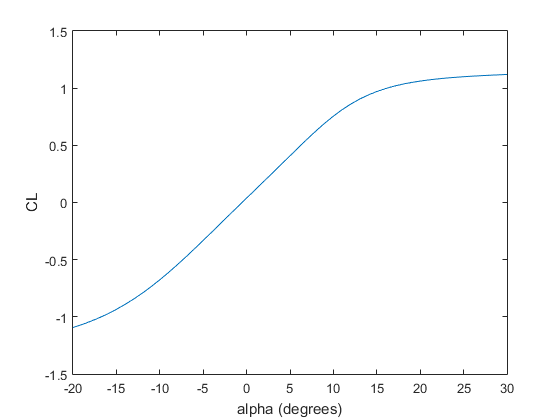
\includegraphics[width=0.75\textwidth]{Figures/CL_alpha.png}
  \caption[$C_L$ versus $\alpha$ graph]{$C_L$ versus $\alpha$ graph from Neural Network}
  \label{fig:cl_alpha}
\end{figure}
From the cruise conditions \ref{eq:cruise_cond}, knowing that $L=\dfrac{1}{2}\rho S V^2 C_L$, solving for the airspeed V comes that

\begin{equation}
V=\sqrt{\dfrac{2mg}{\rho S C_L}}
\label{eq:cruise_speed}
\end{equation}
The required thrust can also be computed from both \ref{eq:cruise_cond}, \ref{eq:cruise_speed} and \ref{eq:cd_cl}, knowing the $C_L$ for a given angle of attack. Proposing some values of $\alpha$, the following results are obtained

\begin{table}[htbp]
  \centering
  \caption{Required cruise conditions for different values of $\alpha$}
    \begin{tabular}{ccccc}
    \toprule
    $\alpha (^o)$ & $C_D$ & $C_L$ & $V (ms^{-1})$ & $T (N)$ \\
    \midrule
    0     & 0.017677131 & 0.0387 & 707.4010791 & 224047.3585 \\
    2     & 0.019379779 & 0.1859 & 322.7613368 & 51133.84325 \\
    4     & 0.023345134 & 0.334 & 240.7952785 & 34283.79709 \\
    6     & 0.029604436 & 0.4828 & 200.279994 & 30076.58604 \\
    \bottomrule

    \end{tabular}
  \label{tab:cruise_cond}%
\end{table}%

From these values, to test both the model (as well as the methods used to simulate the dynamics of the aircraft, including the coefficients neural networks)and the feedback linearisation controller, the following reference values $V_a^d=200 ms^{-1}$, $\gamma^d = 0 rad$ and $\psi^d=0 rad$ were used in an attempt to simulate cruise conditions. From there the values of thrust and angle of attack were computed and  compared to the theoretical values of table \ref{tab:cruise_cond}. 
Following these constant reference values the results obtained were

\begin{figure}
\centering
\begin{minipage}{0.49\textwidth}
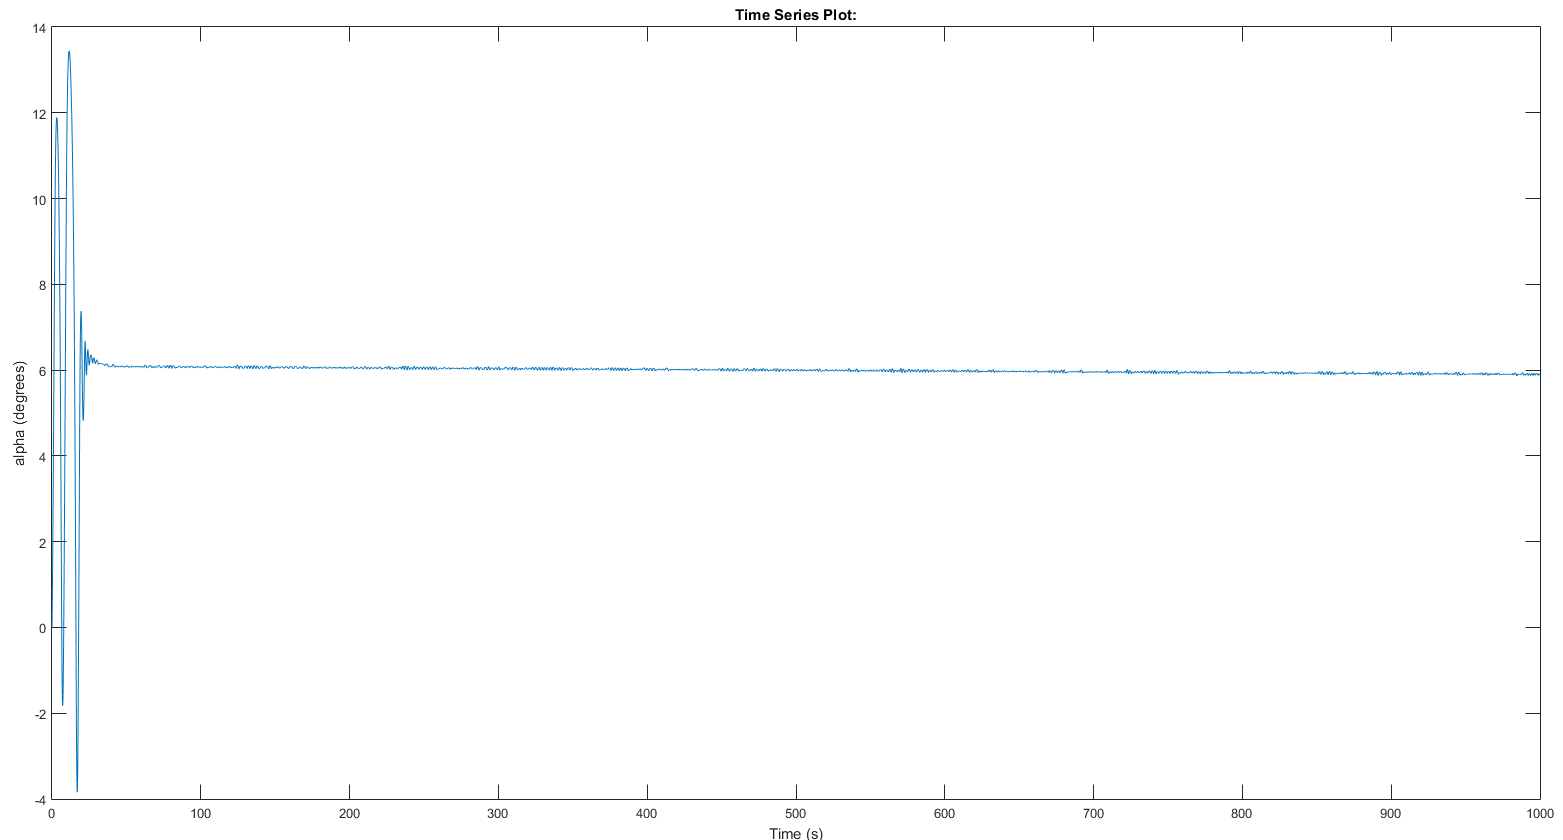
\includegraphics[width=\textwidth]{Figures/Results/aoa_check.PNG}
\end{minipage}
\begin{minipage}{0.49\textwidth}
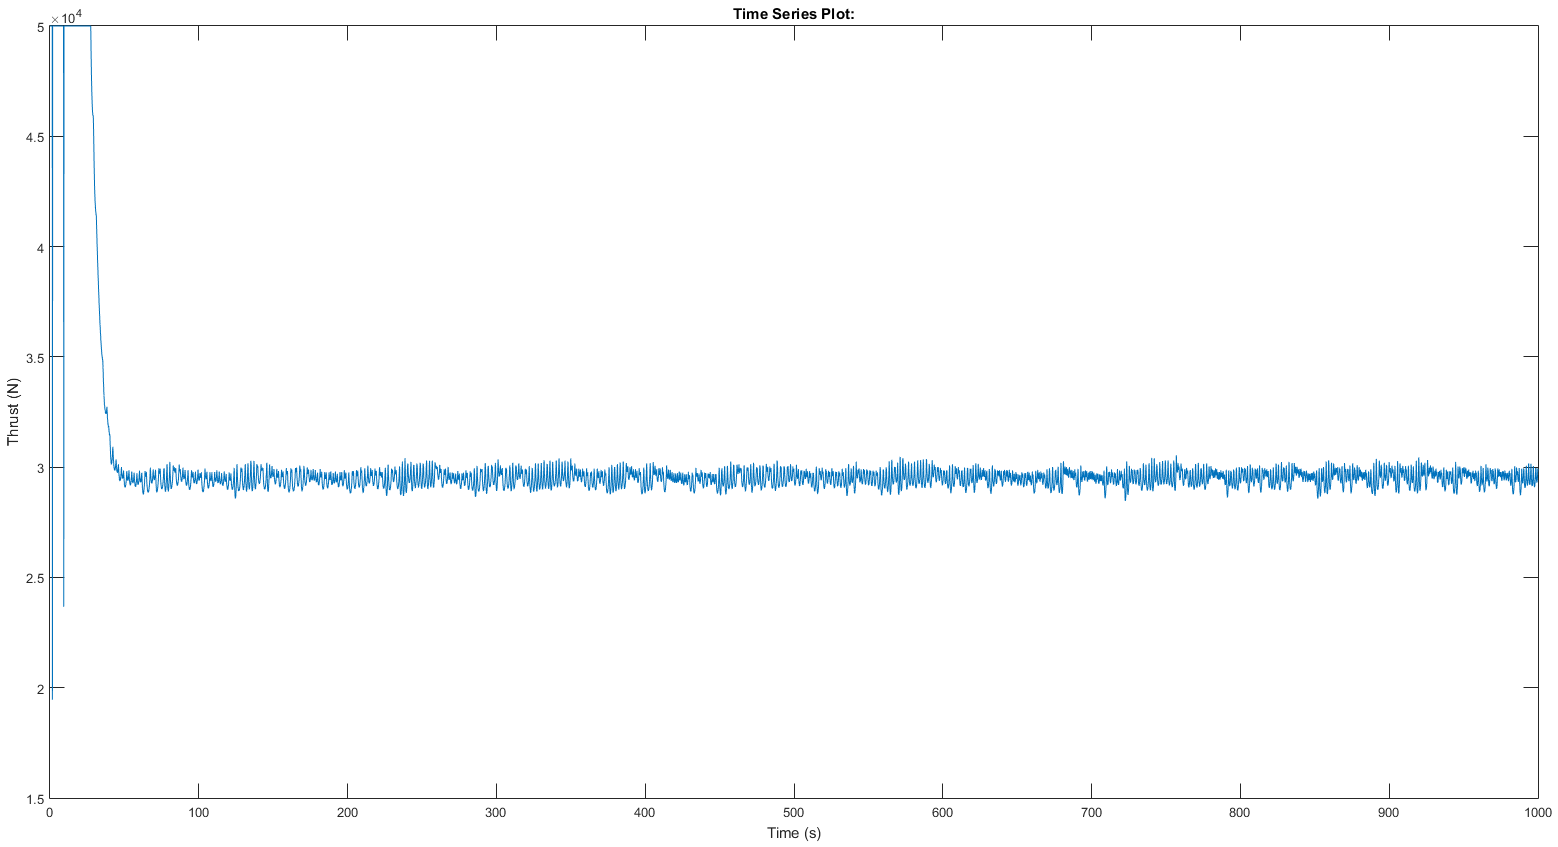
\includegraphics[width=\textwidth]{Figures/Results/thrust_check.PNG}
\end{minipage}
\caption[AoA and thrust validation]{Angle of Attack (degrees) and thrust (N) of the controlled aircraft}
\end{figure}

This simulation, made over 800 seconds, shows clearly that the angle oscillates around a $6^o$ degree angle of attack, with an amplitude of around $0.4^o$ degrees. As for the thrust, it also oscillates around $30000N$ with an amplitude of $2000N$. These values correspond to the theoretical values in table \ref{tab:cruise_cond} for $\alpha=6^o$, indicating that not only the modelled plane is well behaved, but also that the coefficient neural networks are able to simulate an accurate model of the aerodynamic coefficient's variation.


%%%%%%%%%%%%%%%%%%%%%%%%%%%%%%%%%%%%%%%%%%%%%%%%%%%%%%%%%%%%%%%%%%%%%%%%
\section{Feedback linearisation controller}
\label{section:results/fl_contro}

Once the model has been tested and validated, the described nonlinear inversion controller can now be tested. Reference tracking will firstly be observed with simple constant reference values, without any guidance control law. Reiterating the example from the previous section in cruise conditions for $V_a^d=200 ms^{-1}$, $\gamma^d = 0^o$ and $\psi^d = 0^o$ comes that
\begin{figure}[h]
\centering
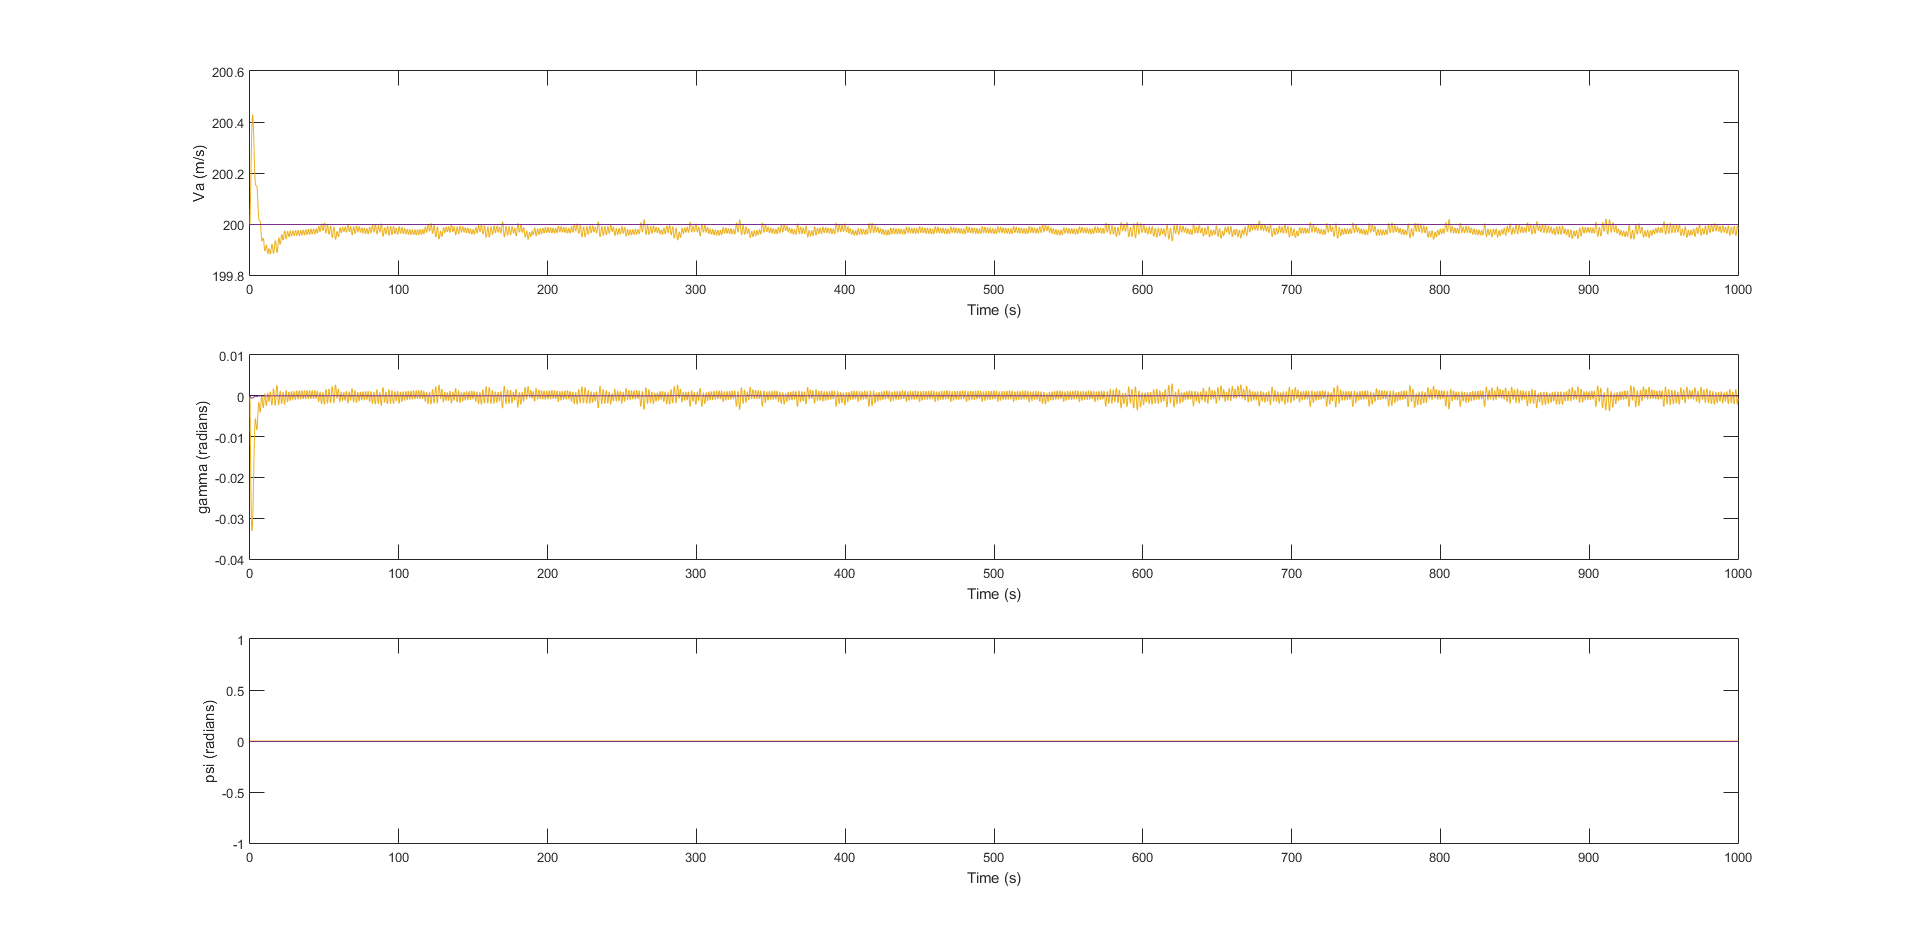
\includegraphics[width=\textwidth]{Figures/Results/nli_test_const.png}
\caption[Constant reference following of feedback linearisation controller]{Reference (blue) following over $1000s$ of simulation time for $V_a^d=200 ms^{-1}$, $\psi^d = 0^o$ and $\gamma^d = 0^o$ respectively and measured values (yellow)}
\label{fig:const_ref}
\end{figure}

As seen in the figure \ref{fig:const_ref} the reference is followed with minimal osculations for the three variables, although with the presence of some steady state error in the case of the airspeed $V_a$. To be able to follow trajectories however, a good control of the aircraft's heading will be necessary. Proposing this time the following variation in $\psi^d$
\begin{equation}
\psi^d = \begin{cases}
0^o & t < 100\\
90^o & 100 \leq t < 500\\
0^o & t > 500 \\
\end{cases}
\label{eq:test_traj}
\end{equation}

The comparing the measured heading $\psi$ and its desired value comes 
\begin{figure}[h]
\centering
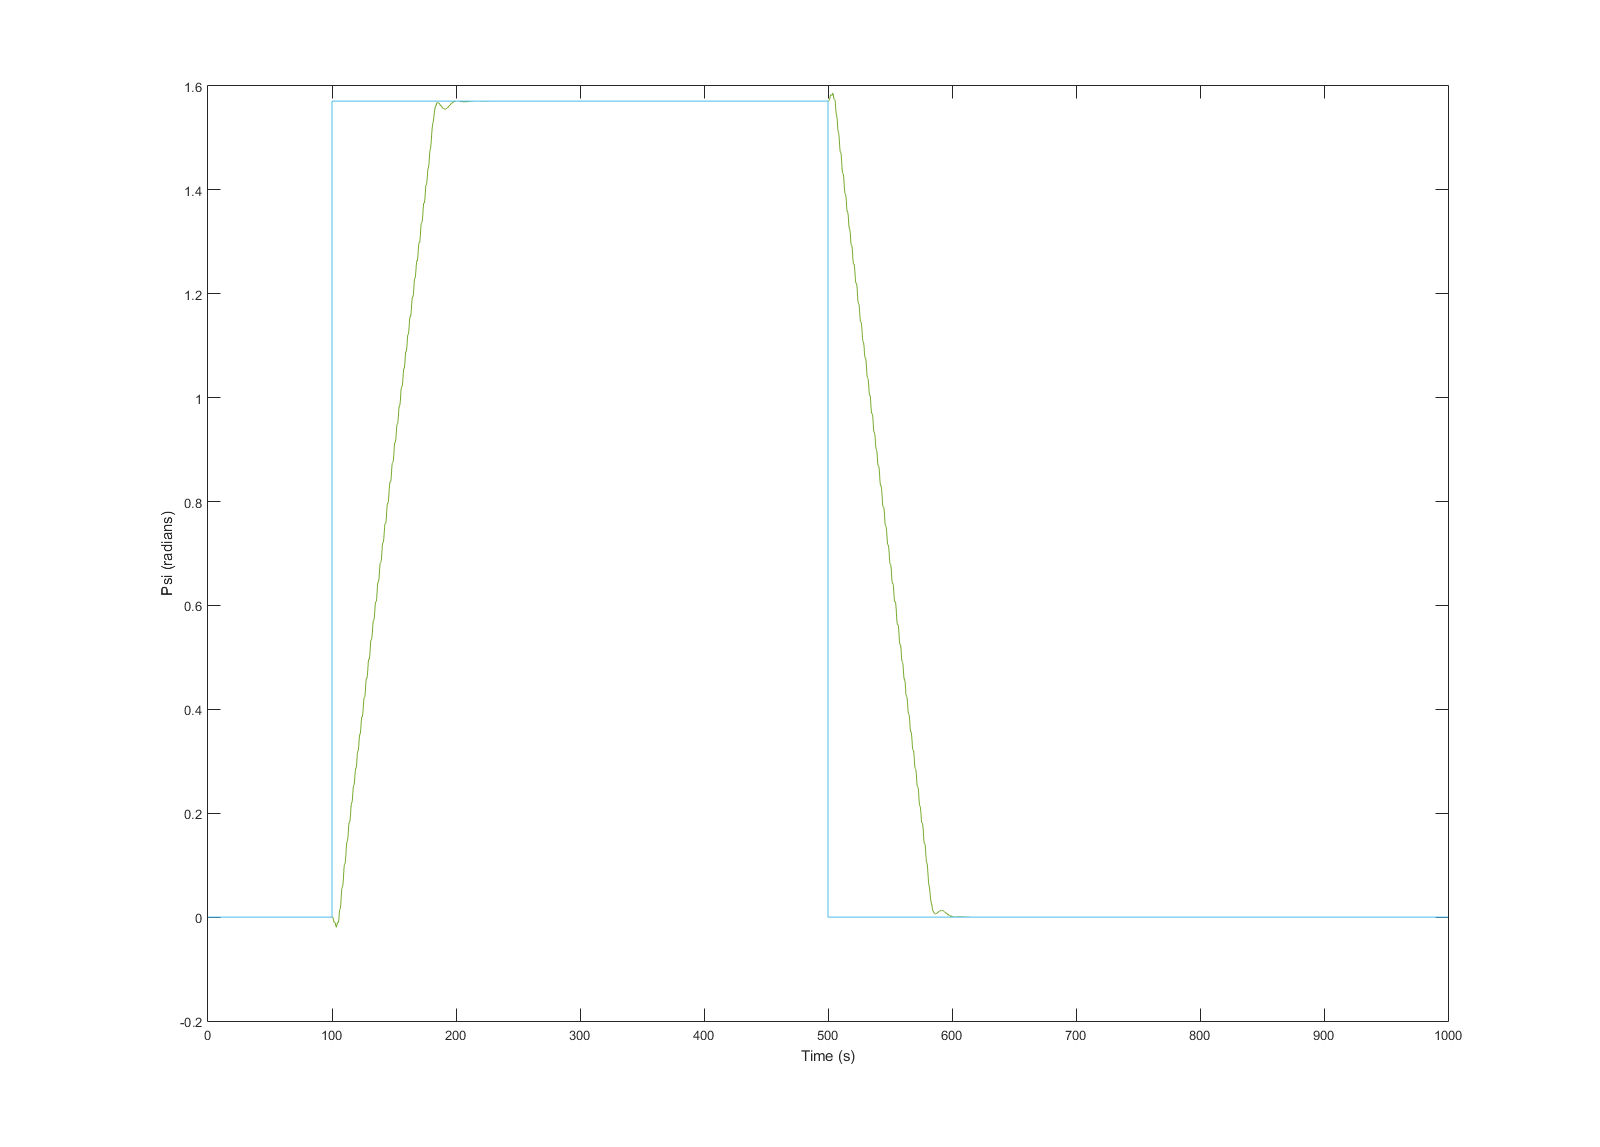
\includegraphics[width=\textwidth]{Figures/Results/heading_test.png}
\caption[Desired and measured heading]{Desired (blue) and measured (green) heading}
\label{fig:heading_test}
\end{figure}

Although the reference value is reached after each step, the convergence takes around $100s$ for a $90^o$ perturbation to converge, without overshoot. These conversion times can be explained by the high inertia and mass of the commercial aircraft. The resulting airplane trajectory can be seen in figure \ref{fig:trajectory}.

\begin{figure}[h]
\centering
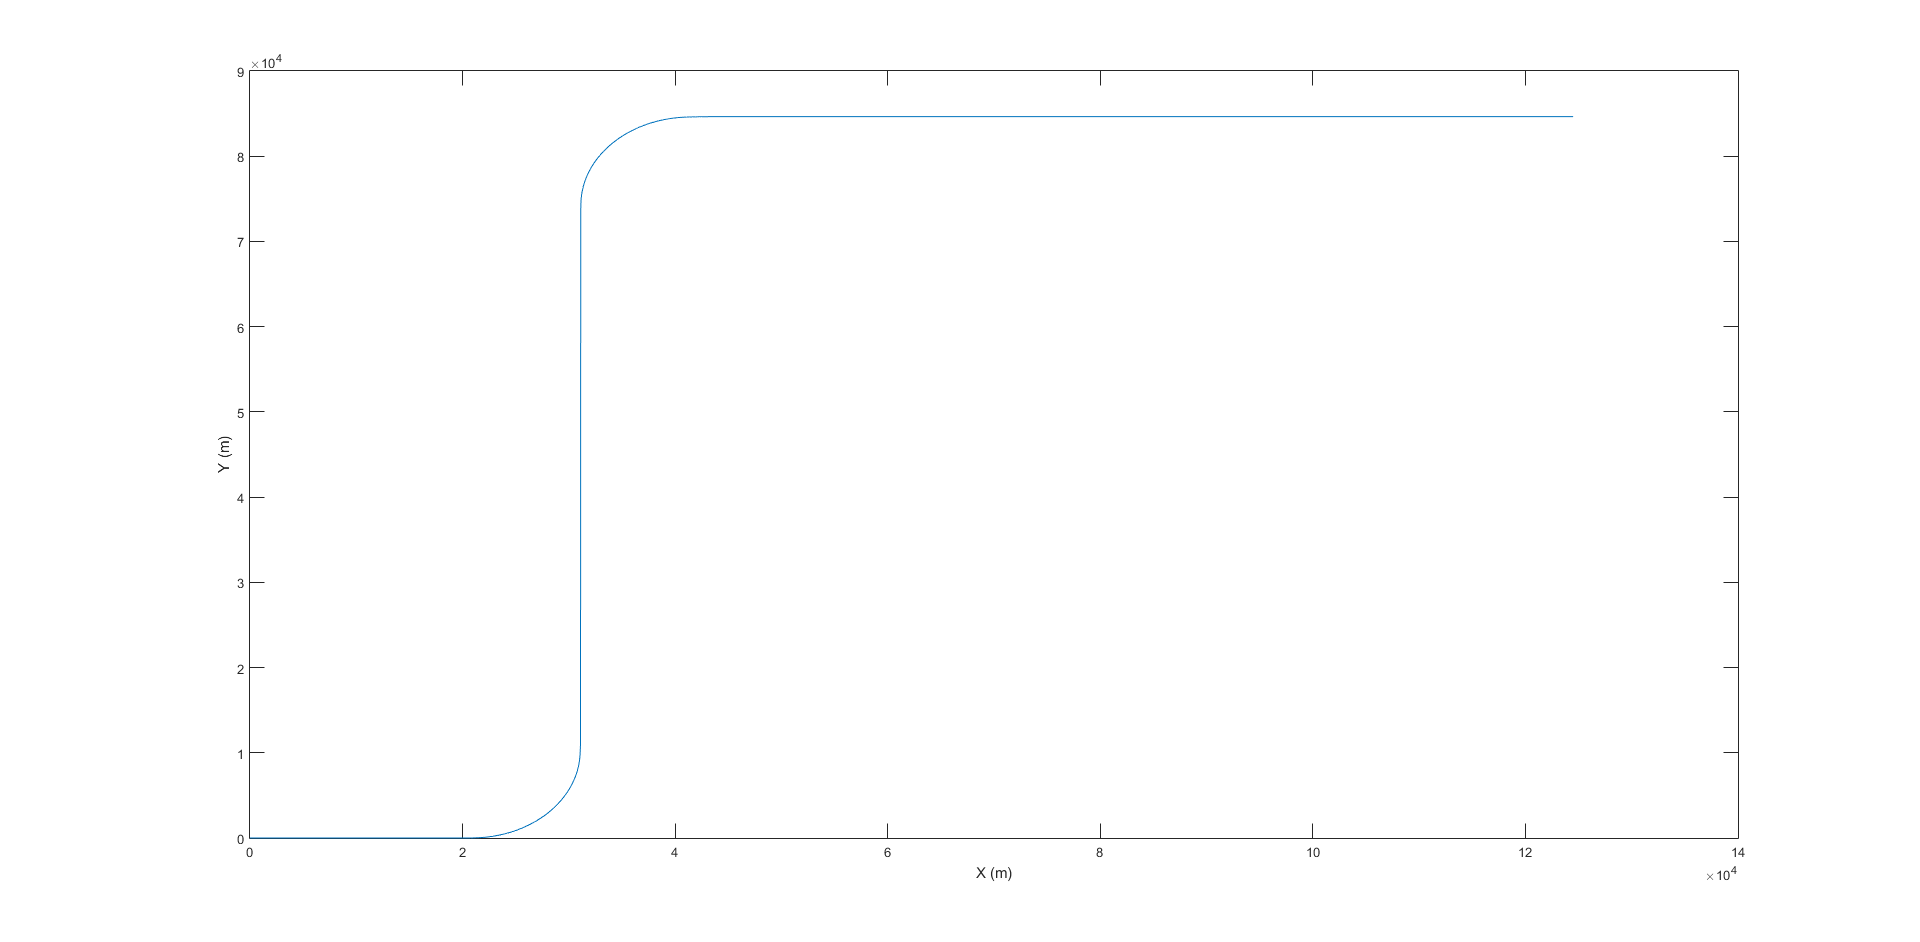
\includegraphics[width=\textwidth]{Figures/Results/trajectory.png}
\caption[Plane trajectory]{Plane trajectory for the mention control input}
\label{fig:trajectory}
\end{figure}

\section{Disturbances and Errors}
\label{section:results/disturbances_errors}

From the results obtained in the previous section, it can be concluded the controller performs correctly following the desired reference. These results however were obtain supposing the exact model of the aircraft was known, without any kind of external perturbation or simulated system failure. It is these perturbations that will be simulated in this section and studied. To do so the same testing reference as described in equation \ref{eq:test_traj} will be used to compare the effects of different types of disturbances with the undisturbed system. 

\subsection{Inversion errors}

This error will be the most frequent when implementing such a controller, as some system parameters estimations may have considerable errors, namely the aircraft's inertial matrix. Fortunately, the controller used is, as will be demonstrated, tolerant to errors in the estimation of this parameter, but can result in an unstable system in extreme cases. To simulate estimation errors, the entries of the inertial matrix $A$,$B$,$C$ and $E$ were multiplied by a reducing factor $\zeta \in [0;1]$ when computing the nonlinear inversion in \ref{eq:control_law}. The inertial matrix used in this equation $I_{est}$ is therefore given by $I_{est} = \zeta I$.

Changing the values of $\zeta$ to $0.5$ and $0.05$, increasing the inversion error, results in the following trajectories in figure \ref{fig:inversion_error}

\begin{figure}[H]
\centering
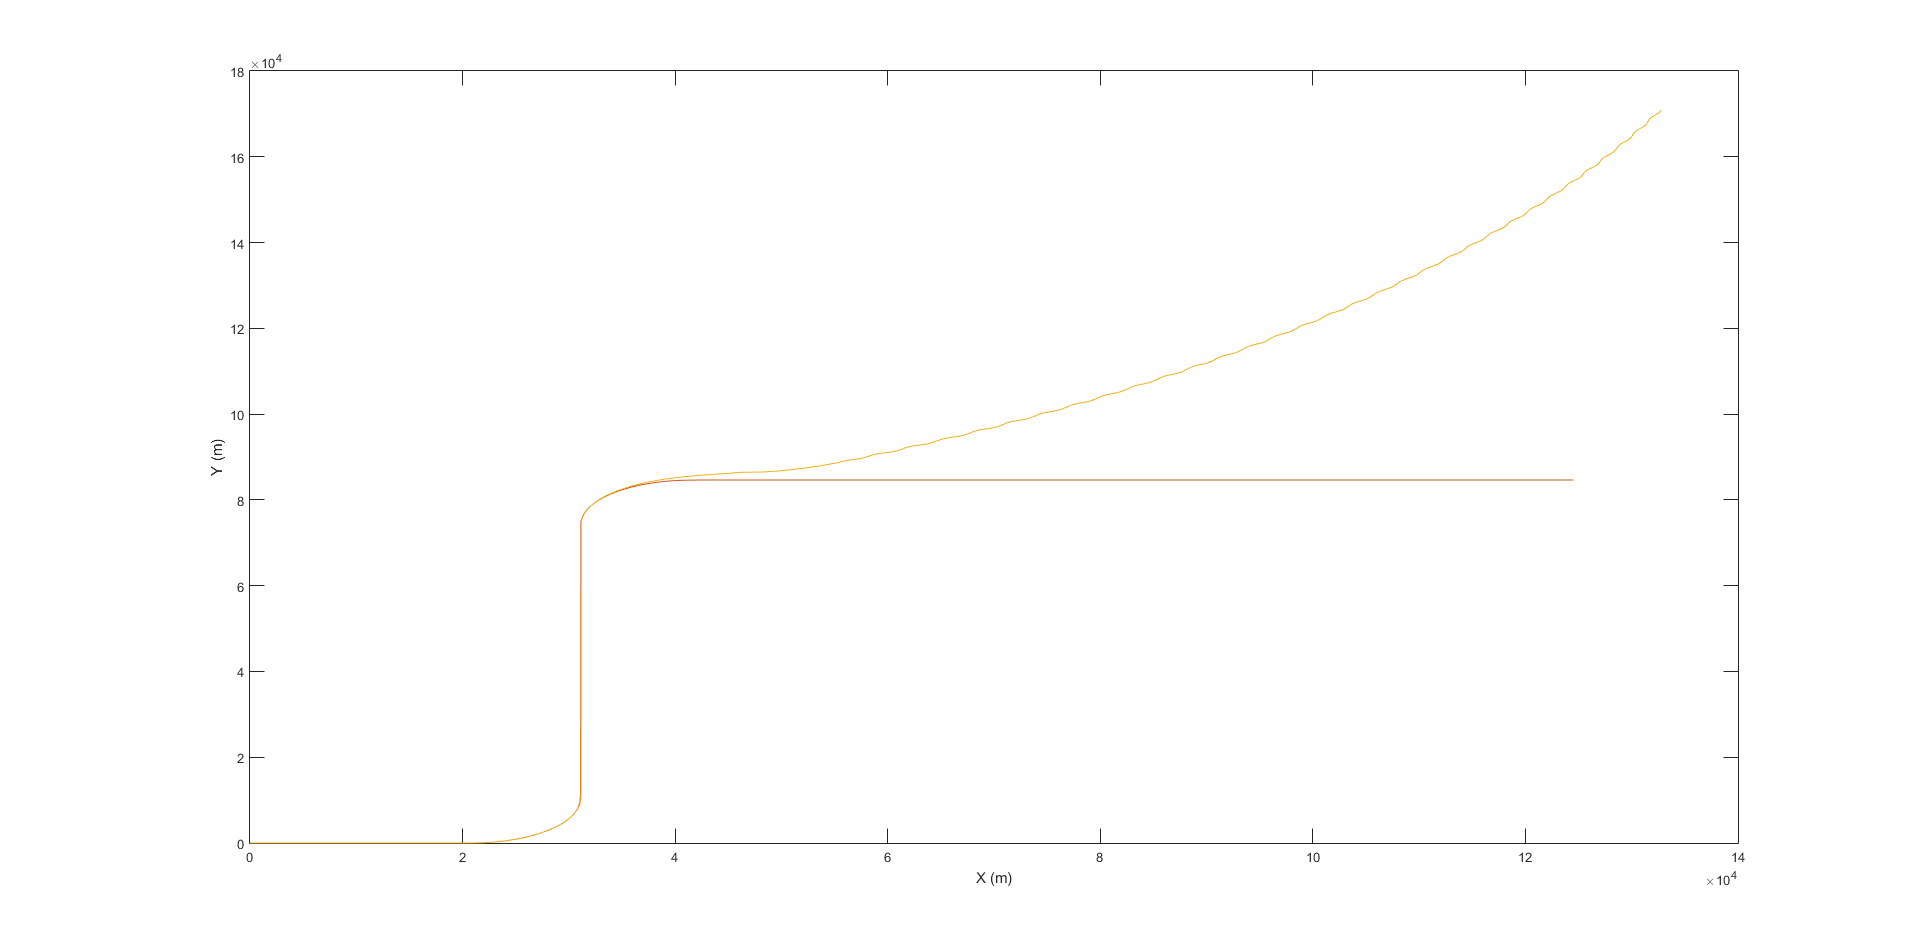
\includegraphics[width=\textwidth]{Figures/Results/inversion_error.png}
\caption[Plane trajectory with inertia estimation errors]{Plane trajectory for for $\zeta = 0.5$ (red) and $\zeta= 0.05$ (yellow)}
\label{fig:inversion_error}
\end{figure}

Indeed, a 50\% error in estimating the inertia of the aircraft when computing the feedback linearisation law results in a negligible reference tracking error, as can be seen in figure \ref{fig:ref_zeta_05}. This however is not the case if $\zeta$ is reduced even further to $\zeta = 0.05$ and error of the system relative to its references becomes much greater (figure \ref{fig:ref_zeta_005}. As can be seen in this figure, the aircraft is unable to follow yaw commands in this case as it easily goes unstable. This establishes a first goal to measure the performance of the designed neural network, to try to approach the case of $\zeta = 0.05$ to the reduced errors of a nonlinear inversion with no inertia estimation errors.

\begin{figure}[H]
\centering
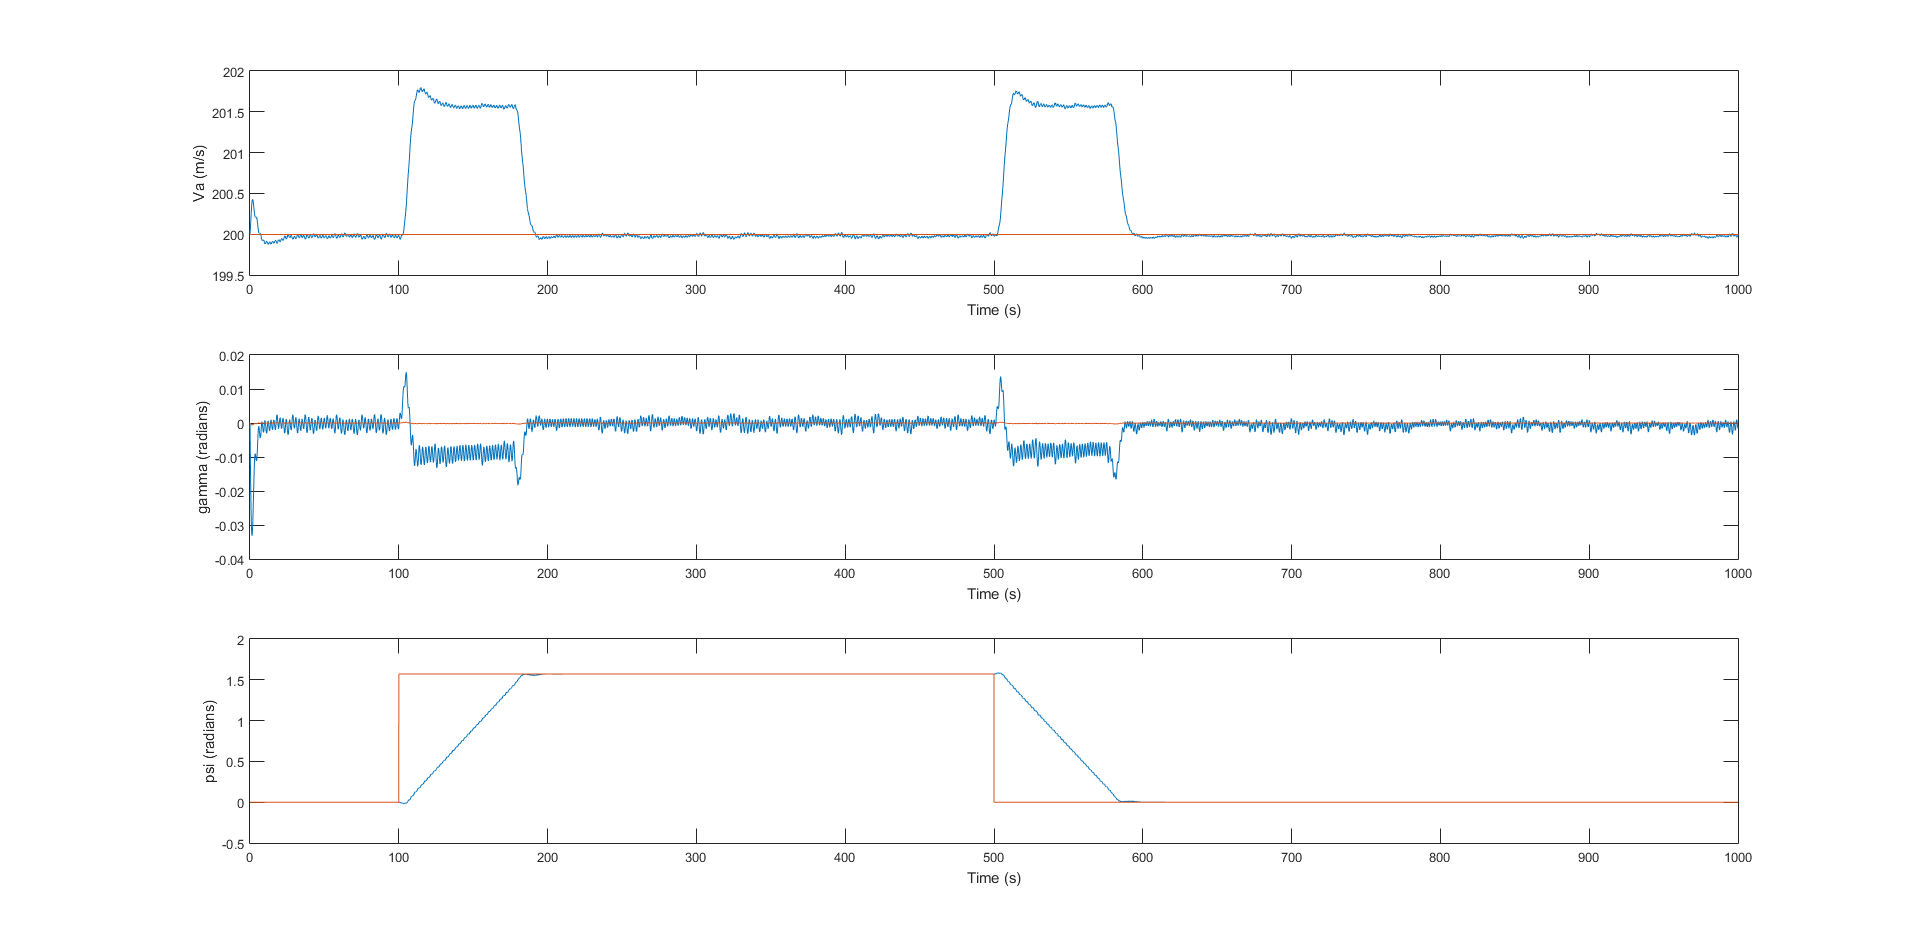
\includegraphics[width=\textwidth]{Figures/Results/ref_zeta_05.png}
\caption[Reference tracking for $\zeta=0.5$]{$V_a$, $\gamma$ and $\psi$ for measured and desired values for $\zeta=0.5$}
\label{fig:ref_zeta_05}
\end{figure}

\begin{figure}[H]
\centering
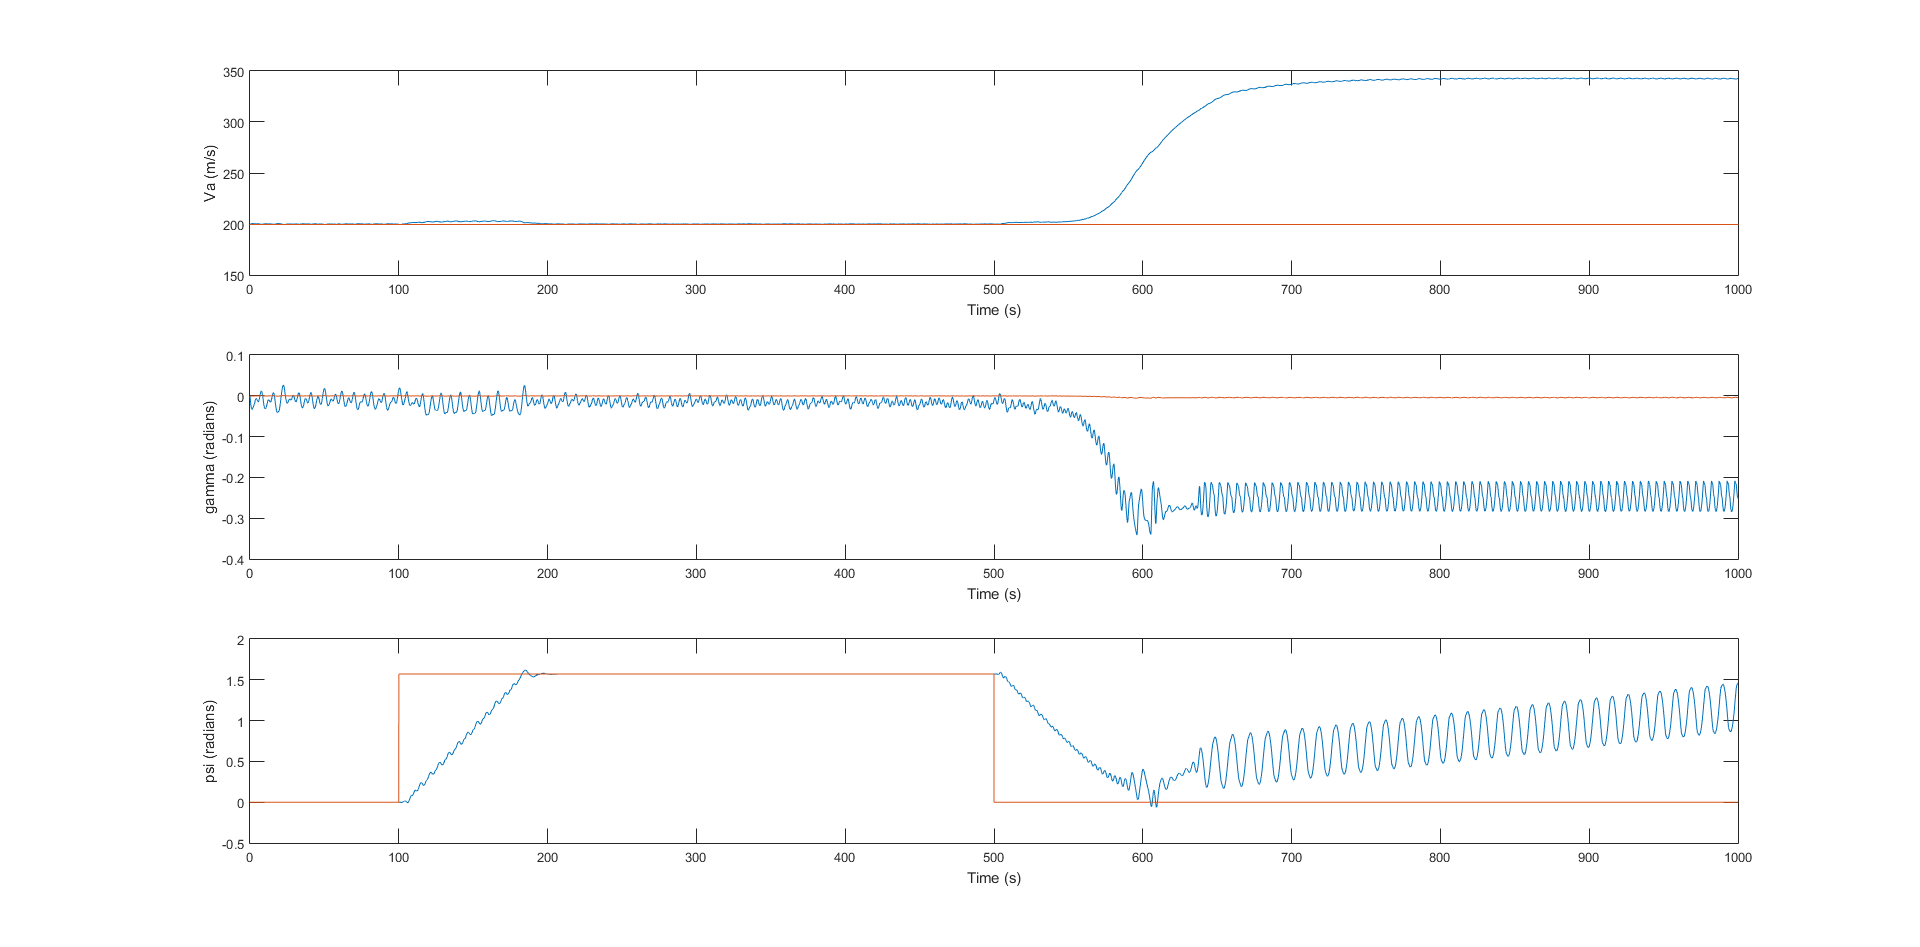
\includegraphics[width=\textwidth]{Figures/Results/ref_zeta_005.png}
\caption[Reference tracking for $\zeta=0.05$]{$V_a$, $\gamma$ and $\psi$ for measured and desired values for $\zeta=0.05$}
\label{fig:ref_zeta_005}
\end{figure}

\subsection{System failures}

One other cause for inversion errors that can have a much greater impact on flight trajectory are system failures. This subsection will focus on methods to simulate these failures and observe the behaviour of the airplane trajectory for these cases. The reference trajectory that will be used shall be the same as used previously. The first failure to be simulated will be a control surfaces failure, that will lead to reduced controllability of the aircraft. In this work this was replicated in a simulated environment by reducing each moment coefficients for the elevon, aileron and rudder, namely $C_{\delta_{ele}}$, $C_{\delta_{ail}}$ and $C_{\delta_{rud}}$.

By setting each of these coefficients to 20\% of their initial values, the effect of the errors in followed trajectory become visible in figure \ref{fig:reduced_act}. This figure show that the reduced controllability results in a $20km$ difference to that of the undisturbed system. This sets the second goal for the performance of the neural network, to reduce this error as much as possible.

\begin{figure}[H]
\centering
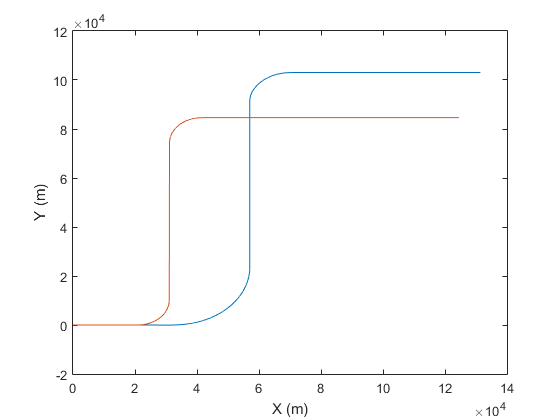
\includegraphics[width=\textwidth]{Figures/Results/reduced_act.png}
\caption[Trajectory with reduced actuation]{Trajectory with 20\% reduced actuation (blue) and trajectory without failures (red)}
\label{fig:reduced_act}
\end{figure}

One second type of flight perturbation that will be included in this subsection is the effects of icing conditions in aircraft flight. According to the FAA guide to flight in icing conditions, ice contamination of an airfoil has an important influence on both the Lift and Drag curves \cite{icing_cond}. Ways to simulate these perturbations in a modelled environment will be studied, and as for the the other described disturbances an online neural network will be used to improve the control of the aircraft in such conditions. The main drawbacks that can be caused by icing are

\begin{itemize}
\item \textbf{Stall }As seen in figure \ref{fig:icing_lift}, ice contamination of the airfoil leads to a significant reduction in the value of the maximum $C_L$, causing the aircraft to reach stall conditions ata much lower angle of attack. Reducing speed (e.g for an approach) makes this effect more noticeable for the pilot. The usual reduction on $C_{L_{max}}$ is of 30\% \cite{icing_cond}.

\item \textbf{Drag }Drag will increase directly with the amount of ice accumulated on the wing, reaching usual values of 100\% of the initial drag coefficient.

\item \textbf{Roll }Icing on the main wings will also affect roll control. As the thickness of the wing decreases towards its tip, so increases its efficiency to collect ice, leading to a partial stall in the tip of the wings. 
\end{itemize}
\begin{figure}[H]
\centering
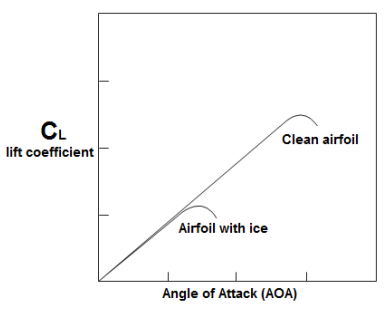
\includegraphics[width=0.7\textwidth]{Figures/Results/icing_lift.PNG}
\caption[Effects of icing on the lift coefficient]{Effects of icing on the lift coefficient \cite{icing_cond}}
\label{fig:icing_lift}
\end{figure}
\begin{figure}[H]
\centering
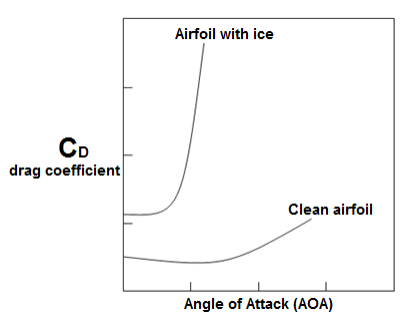
\includegraphics[width=0.7\textwidth]{Figures/Results/icing_drag.PNG}
\caption[Effects of icing on the drag coefficient]{Effects of icing on the drag coefficient \cite{icing_cond}}
\label{fig:icing_drag}
\end{figure}
\subsection{Wind disturbances}

TODO?

\section{Neural Network}
\label{section:results/NN}

\section{Guidance controller}
\label{section:results/guidance_control}


